%% ==============================
\chapter{\iflanguage{ngerman}{Konzept}{Technogical Fundations}}
\label{sec:Technogical Fundations}
%% ==============================
This chapter introduces technological foundations fundamental for this thesis, which includes methods, models and tools that are used later in the thesis. The first section focus on the basic principle of Unity3D, which is used to build simulation environment for generating synthetic images. Then the second section shortly explain the essential knowledge of deep learning, especially convolution neural network(CNN), which used by modeling to recognize objects and predict the 3D-pose of them. Section 2.2 give an overview of the Kreas/Tensorflow framework, which will be used for training the CNN-model. Section 2.3 shows how to build a shallow neural network model in Keras and train it.

\section{Unity3D background}
Unity is a cross-platform game engine developed by Unity Technologies. Due to the motivation of transfer learning from simulation to real environment, a simulation scene in virtual environment need to be built and large numbers of synthetic image data of it are requisite. The unity engine gives users the ability to create virtual objects in 3D and offers a primary scripting API in C\# to render images that are needed in this research. All these features shows that Unity is suitable for rendering requests and can simplify the works during modeling. 
\subsection{User interface}
Unity provides a basic graphical interface to build the simulation environment, which includes five basic windows. 
\begin{itemize}
	\item The Scene View: where user work with game objects, including models, lights and colliders, to construct the user's scenes. 
	\item The Game View: where user can preview and play simulation scene as a work in progress as user develop it.
	\item The hierarchy window: All of the game objects in the open scenes are listed by the hierarchy window in hierarchical order.
	\item The project window: where user imports, stores and edits the Asset files. 
	\item The inspector window: It is context sensitive and displays all the properties of any selected game object, asset or setting.
\end{itemize} 
All the modeling works can be done in the graphical user interface. A general method of modeling are divided into 4 steps. Firstly a new default model needs to be created in Unity or imported from other 3D modeling software. This new model will appear in hierarchy window with other existent objects. Here the hierarchical relations can be adjusted. Secondly the dimensions and positions of new created model can be modified in inspector window, and new components (e.g. C\# scripts, Mesh Renderer, etc.) can be added into the model. Then in scene window a arbitrary perspective could be set, and according to the local coordinate system the position relationship among different objects can be adjusted. Finally when all items are correctly set and all needed components are added on them, the simulation scene can be played and the progress can be monitored in game view window in real time.
\subsection{Coordinate system in Unity}
The world coordinate system is left handed (as Direct X) where x positive axis is right, y positive is up and z is positive into the screen.\\
\begin{figure}[h]
	\centering
	\captionsetup{justification=centering}
	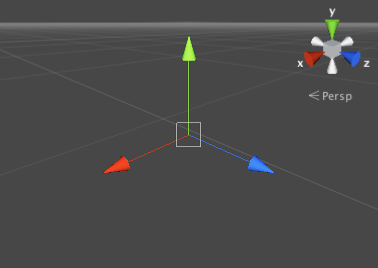
\includegraphics{{Figures/Section3_CoordinateSystem.png}}
	\caption{Coordinate system in Unity}
	\label{fig: Coordinate unity}
\end{figure}\\
Screen coordinate system is bottom-up: (0,0) at bottom-left corner and (pixelWidth-1,pixelHeight-1) at right-top; x axis is positive right and y is positive up. The z position is in world units from the camera.\\
Viewport coordinate system is normalized and relative to the camera, so the bottom-left point is (0,0), the top-right is (1,1). The z position is in world units from the camera.\\
Finally UI coordinate system is top-down: the y coordinate varies from zero at the top edge of the window to a maximum at the bottom edge of the window. The upper-left point is (0,0); the bottom-right is (1,1).\\
There are many functions to convert between all these different coordinate systems
\subsection{Basic concepts in scene}
To build a basic scene in Unity 3D, some important core concepts need to be known. which include Game Object, Component, Script and etc. They form the main basic elements of unity and should be added into the scene to realize the needed functions and effects. Normally the Component and Script are sub-element of the Game Object.\\
\begin{itemize}
	\item Scenes: Scenes contain the objects of simulation project. They can be used to create a main menu, individual levels, and anything else. Each unique Scene file is a unique level. In each Scene, the environments, obstacles, decorations will be placed, and the project are designed and built in pieces.\\
	A new Unity project will show a new Scene. The scene will be empty except for default objects- either an orthographic camera, or a  perspective camera and a directional light. 
	\item GameObjects: The GameObject is the most important concept in the Unity Editor.\\
	Every object in project is a GameObject. This means that everything which can be thought of to be in the project has to be a GameObject. However, a GameObject can't do anything on its own; The properties need to be given before it can become a character, an environment, or a special effect.\\
	A GameObject is a container; pieces are added to the GameObject container to make it into a character, a light, or whatever needed in project. Each added piece is called a component.\\
	Depending on what kind of object need to be created, different combinations of components can be added to a GameObject. A GameObject could be thought of as an empty cooking pot, and components are different ingredients that make up the recipe of project.  
	\item Component: Components are the nuts \& bolts of objects and behaviors in a game. They are the functional pieces of every GameObject.\\
	A GameObject is a container for many different Components. By default, all GameObjects automatically have a Transform Component. This is because the Transform dictates where the GameObject is located, and how it is rotated and scaled. Without a Transform Component, the GameObject wouldn't have a location in the word.
	\item Script: Scripting is an essential ingredient in all projects. They can be used to create graphical effects, control the physical behavior of objects and even implement a custom automatic system in the project. In next subsection, basic knowledge of scripting will be introduced to show how the script runs in unity and which basic functions are included in it. 
\end{itemize}
\subsection{Basic knowledge of script}
Unity supports the C\# programming language, which is an industry-standard language similar to Java or C++.\\
A script makes its connection with the internal workings of Unity by implementing a class which derives from the built-in class called MonoBehaviour. A class is like a kind of blueprint for creating a new Component type that can be attached to GameObjects. The core elements to realize different effects are the Event Functions. A script in Unity is not like the traditional idea of a program where the code runs continuously in a loop until it completes its task. Instead, Unity passes control to a script intermittently by calling certain functions that are declared within it. Once a function has finished executing, control is passed back to Unity. These functions are known as event functions since they are activated by Unity in response to events that occur during gameplay. Unity uses a naming scheme to identify which function to call for a particular event. There are four basic types of events:
\begin{itemize}
	\item Regular Update Events: 
	\begin{enumerate}
		\item Update function: The Update function is the main place for making changes to position, state and behavior of objects in the scene just before each frame is rendered. Update is called before the frame is rendered and also before animations are calculated.
		\item FixedUpdate function: The physics engine also update in discrete time steps in a similar way to the frame rendering. A separate event function called FixedUpdate is called just before each physics update.
		\item LateUpdate function: It is also useful sometimes to be able to make additional changes at a point after the Update and FixedUpdate functions have been called for all objects in the scene and fter all animations have been calculated.
	\end{enumerate}
	\item Initialization Events:
	\begin{enumerate}
		\item Start function: It is called before the first frame or physics update on an object.
		\item Awake function: The Awake function is called for each object in the scene at the time when the scene loads. All the Awakes will have finished before the first Start is called. This means that code in a Start function can make use of other initializations previously carried out in the Awake phase.
	\end{enumerate}
	\item GUI event: Unity has a system for rendering GUI controls over the main action in the scene and responding to clicks on these controls. This code is handled somewhat differently from the normal frame update and so it should be placed in the OnGUI function, which will be called periodically.
	\item Physics events: The physics engine will report collisions against an object by calling event functions on the object's script. 		
\end{itemize}
\begin{figure}[h]
	\centering
	\captionsetup{justification=centering}
	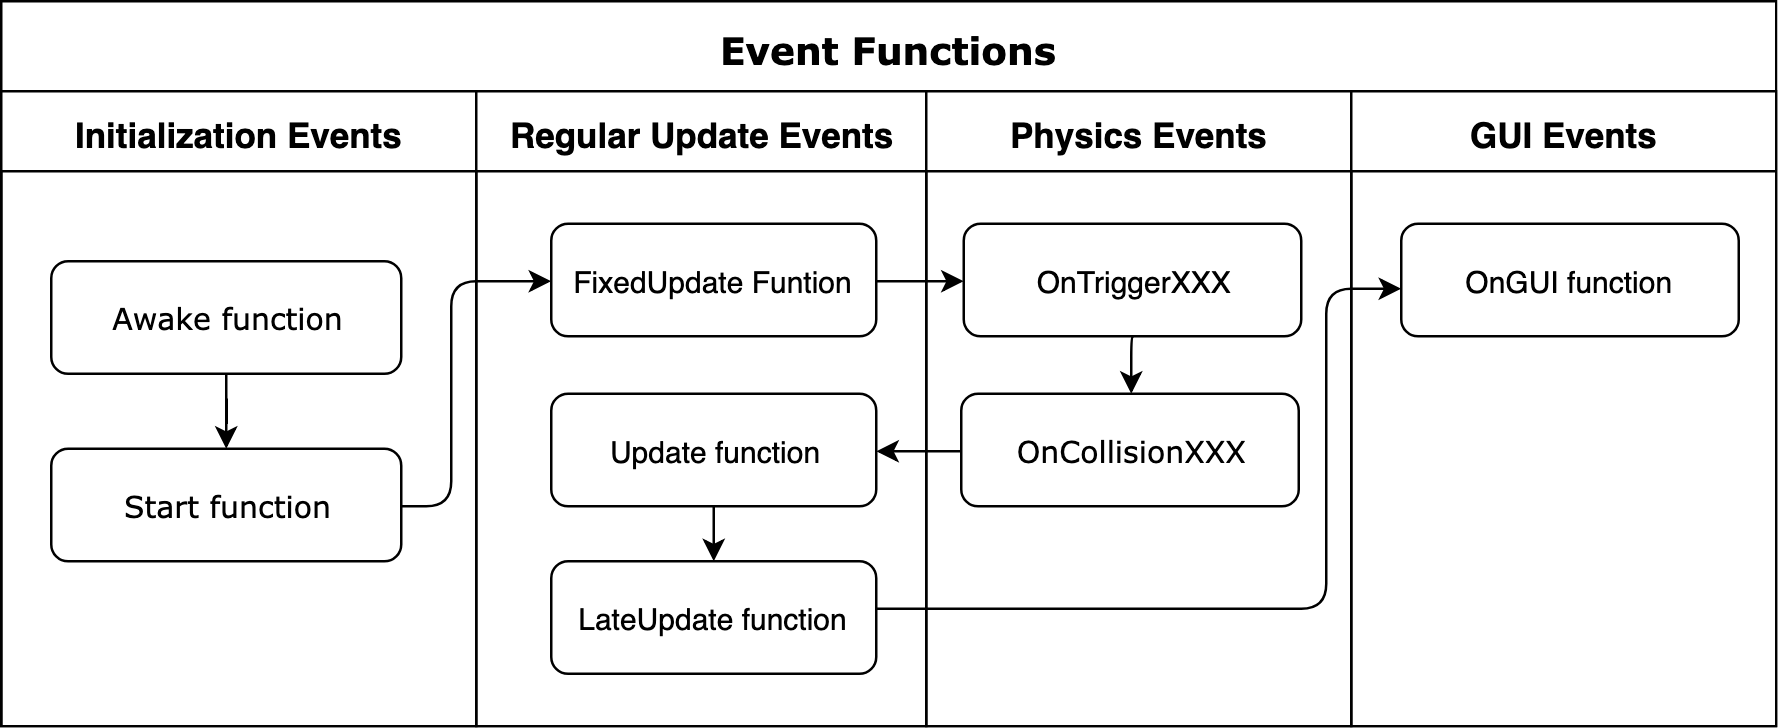
\includegraphics[width=\textwidth]{Figures/Section3_Eventfunction.png}
	\caption{Event function and execution order in Unity}
	\label{fig: event_function}
\end{figure}

\section{Neural network and Deep Learning}
\subsection{title}
